\documentclass[oneside,12pt]{wipb}
\usetikzlibrary{mindmap,trees}%dla diagramu Computer science mindmap


\katedra{Oprogramowania}
\typpracy{ in?ynierska
           %in�ynierska
         }
\temat{Aplikacja internetowa do obs?ugi systemu
GDT w technologii Python/Django}
\autor{Gal Anonim}
\promotor{Juliusz Cezar}
\indeks{123456}
\studia{stacjonarne
        %niestacjonarne
       }
\rokakademicki{2008/2009}
\profil{studia I stopnia}
\kierunekstudiow{informatyka}
%\specjalnosc{In�ynieria Oprogramowania
             %In�ynieria Komputerowa
             %Systemy Oprogramowania
             %Metody infnformatyczne w~banknkowo�ci i~finansach
             %Ochrona system�w informatycznych
 %   }
\zakres{1. zakres I \newline 2. zakres II \newline 3. zakres III}

\hypersetup{ %wpisy w pdf info
pdfauthor={ Mateusz Pernal},
pdftitle={Praca inzynierska},
pdfsubject={},
pdfkeywords={Praca inzynierska},
pdfpagemode=UseNone,
linkcolor=black,
citecolor=black
} 

\begin{document}
\maketitle
\tableofcontents
\thispagestyle{empty}
\setcounter{page}{0}
\pagestyle{plain}
\chapter{Architektura rozwiązania}
\section{Architektura aplikacji}
Struktura aplikacji jest oparta na podziale wynikającym z wykorzystania frameworka Django. Zgodnie z tym założeniem projekt dzieli się na poszczególne moduły, które w rozumieniu platformy nazywane są paczkami.  W aplikacji można wyróżnić cztery podstawowe elementy kolejno odpowiadające za zarządzanie eksperymentami i użytkownikami, interfejs graficzny oraz aplikacja zbierająca wszystko w całość. Schemat modułów jest przedstawiony na Rys. \ref{rys4_packages}. 

Aplikacja jest zaimplementowana zgodnie ze stylem architektonicznym REST (\textit{Representational State Transfer}). Architektura ta jest bardzo popularna przy tworzeniu aplikacji internetowych ze względu na swoją lekkość oraz prostotę. Do komunikacji pomiędzy widokami aplikacji, a logiką biznesową znajdującą się na serwerze, wykorzystywany jest protokół http. W tym celu do każdej poszczególnej funkcjonalności działającej w projekcie musiał zostać wystawiony endpoint. Zbiór wszystkich wystawionych serwisów przyjmuje nazwę API \textit{(Application Programming Interface)}. Taki rodzaj rozwiązania zapewnia jasny podział na poszczególne warstwy, które są od siebie niezależne. Dzięki temu część serwerowa aplikacji może działać nie ingerując w część interfejsu graficznego. Mapowaniem poszczególnych modułów aplikacji na endpointy zajmuje się główna aplikacja \enquote{decisionTree}. 


Obok plików aplikacji można wyróżnić folder \enquote{users} zawierający foldery użytkowników. Nazwy tych katalgów są tworzone na bazie loginu. Każdy użytkownik może wgrywać dowolną ilość plików o rozszerzeniach \enquote{*.xml}, \enquote{*.data}, \enquote{*.test} oraz \enquote{*.names} do swojego folderu. Podczas tworzenia nowego eksperymentu tworzony jest dla niego katalog o nazwie składającej się z pola  \enquote{id} i \enquote{name}. Tam są przechowywane wszystkie pliki  związane z doświadczeniem. Użytkownik ma możliwość pobrania całego folderu z plikami eksperymentu w postaci archiwum o rozszerzeniu  \enquote{*.zip}. Dodatkowo w aplikacji jest dostępna opcja zarządzania katalogiem głównym użytkownika. Udostępnione są opcje do zmiany nazwy, usunięcia czy też pobrania pliku. 

\begin{figure}[htb]
	\centering
	\includegraphics[height=8cm]{grafika/packages.eps}
	\caption{Podział projektu na moduły, źródło: opracowanie własne}
	\label{rys4_packages}
\end{figure}
%\subsection{Generowanie postępu}
Użytkownik uruchamiając nowy eksperyment, powinien widzieć jego postęp, jak i średni czas, który pozostał do końca. Zostało to rozwiązane w aplikacji po przez tabelę w bazie pośredniczącą wymianie informacji o progresie doświadczania. Program uruchomiony w robotniku Celery, wypisuje informacje na standardowe wyjście (stdin). W tych danych znajduje się numer iteracji wykonanej oraz średni jej czas. Stosując połączenie za pośrednictwem PIPE, robotnik może przeanalizować te informacje. W celu ograniczenia obciążenia co dziesiąta linia jest poddawana analizie. Na podstawie zawartych tam danych oraz ilości uruchomień algorytmu uzyskanej z pliku konfiguracyjnego można wyliczyć średni czas pozostały do końca obliczeń. Natomiast pasek postępu zostaje wyznaczony poprzez określenie numeru ostatniej iteracji i stwierdzeniu ile wykonań algorytmu jeszcze pozostało. 

%\subsection{Autoryzacja użytkownika}
Autoryzacja użytkowników jest nieodłącznym elementem aplikacji internetowej. W tym celu został wykorzystany mechanizm tokenów. Taki token jest przyznawany dla użytkownika po zalogowaniu lub samej rejestracji. Umożliwia on autoryzowany dostęp do strony internetowej i jest przekazywany w każdym zapytaniu. Po stronie wizualnej aplikacji jest przechowywany w \textit{local storage} przeglądarki internetowej. Każdy token posiada swój czas aktywności, a po jego wygaśnięciu lub przy dowolnym problemie z jego uwierzytelnieniem użytkownik zostanie przekierowany na stronę główną. 

\section{Przechowywanie danych}
W celu przechowywania wszelkich informacji została wykorzystana relacyjna baza danych PostgresSQL. Platforma ta jest postawiona na oddzielnym kontenerze w celu uzyskania większej stabilności i nie zależności od głównego modułu aplikacji. Schemat struktury wszystkich tabel został przedstawiony na Rys. \ref{rys5_database_schema}. Większość tabel wynika z samego zastosowania frameworka Django i DjangoRestFramework. Wykorzystując gotowe rozwiązana zostały zapewnione takie modele jak \enquote{auth\_user} odpowiadający za zapisywanie informacji o użytkownikach, czy też \enquote{authtoken\_token} mająca na celu przetrzymywanie tokenów autoryzacji. Do całej struktury zostały dodane dodatkowe tabele:
\begin{itemize}
	\item \enquote{decisionTreeCore\_experiment} przetrzymująca dane o eksperymentach,  
	\item \enquote{decisionTreeCore\_permissions} zawierająca informacje o prawach dostępowych do eksperymentu,
	\item \enquote{decisionTreeCore\_progress} składa się z pól określających postęp wykonywania doświadczenia.
\end{itemize}



\begin{figure}[htb]
	\centering
	\includegraphics[angle=270, width=16cm]{grafika/database_schema.eps}
	\caption{Schemat bazy danych, źródło: opracowanie własne}
	\label{rys5_database_schema}
\end{figure}

 
\begin{figure}[htb]
	\centering
	\includegraphics[height=16cm]{grafika/database_schema_2.eps}
	\caption{Schemat tabel dodatkowych, źródło: opracowanie własne}
	\label{rys6_database_schema}
\end{figure}

\begin{table}[htb]
	\centering
	\begin{tabular}{|c|c|p{9cm}|}
		\hline
		\textbf{Nazwa pola} & \textbf{Typ} & \textbf{Opis} \\\hline
		id & integer & Klucz główny tabeli \\\hline
		name & varchar(50) & Nazwa eksperymentu\\\hline
		description & varchar(250) & Opis eksperymentu\\\hline
		error\_message & varchar(250) & Wiadomość o błędzie, który wystąpił podczas uruchomienia eksperyment\\\hline
		status & varchar(15) & Pole określające w jakim statusie znajduje się eksperyment. Możliwe wartości to: \enquote{Created}, \enquote{In queue}, \enquote{Running}, \enquote{Finished}, \enquote{Error}. Zmiana statusów następuje w trakcie przechodzenia eksperymentu przez kolejne etapy\\\hline
		data & datetime & Data stworzenia eksperymentu przez użytkownika\\\hline
		config\_file\_name & varchar(50) & Nazwa pliku konfiguracyjnego użytego w eksperymencie\\\hline
		data\_file\_name & varchar(50) & Nazwa pliku zawierającego zbiór uczący \\\hline
		test\_file\_name & varchar(50) & Nazwa pliku zawierającego zbiór testowy \\\hline
		names\_file\_name & varchar(50) & Nazwa pliku określającego nazwy klas oraz rodzaj zmiennych \\\hline
		result\_directory\_path & varchar(50) & Ścieżka do folderu z wynikami eksperymentu\\\hline
		user\_id & integer & ID użytkownika, który jest właścicielem eksperymentu \\\hline
		runs\_number & smallint & Pole określające ile przebiegów algorytmu ma się odbyć podczas uruchomienia eksperymentu w systemie GDT. Pełni ważną rolę przy tworzeniu paska postępu oraz określeniu liczby wyświetlanych drzew\\\hline
		task\_id & varchar(250) & Zawiera id zadania, które trafiło do robotnika Celery. Umożliwia zarządzanie danym zadaniem np. usunięcie z kolejki, lub anulowanie w trakcie trwania\\\hline
		shared\_from & varchar(250) & Pole pełni rolę zapisu informacji o poprzednich właścicielach. W wartością pola są nazwy użytkowników. Podczas kolejnych udostępnień do pola są dodawane po przecinku następne loginy  \\\hline
	\end{tabular}
	\caption[Opis pól encji \enquote{decisionTreeCore\_experiment}]{ Opis pól encji \enquote{decisionTreeCore\_experiment}}
	\label{tabela_1_schema_experiment}
\end{table}

\begin{table}[htb]
	\centering
	\begin{tabular}{|c|c|p{9cm}|}
		\hline
		\textbf{Nazwa pola} & \textbf{Typ} & \textbf{Opis} \\\hline
		id & integer & Klucz główny tabeli \\\hline
		iteration & integer & Liczba iteracji eksperymentu\\\hline
		last\_iter\_number & integer & Numer ostatniej iteracji\\\hline
		mean\_time & real & Wiadomość o błędzie, który wystąpił podczas uruchomienia eksperyment\\\hline
		experiment\_id & integer & Numer id eksperymentu, do którego jest przypisany postęp \\\hline
		run\_number & integer & Numer określający, które uruchomienie algorytmu właśnie trwa\\\hline
		
	\end{tabular}
	\caption[Opis pól encji \enquote{decisionTreeCore\_progress}]{ Opis pól encji \enquote{decisionTreeCore\_progress}}
	\label{tabela_2_schema_progress}
\end{table}

\begin{table}[htb]
	\centering
	\begin{tabular}{|c|c|p{9cm}|}
		\hline
		\textbf{Nazwa pola} & \textbf{Typ} & \textbf{Opis} \\\hline
		id & integer & Klucz główny tabeli \\\hline
		run & bool & Prawo do uruchamiania eksperymentu\\\hline
		edit & bool & Prawo do edycji\\\hline
		download\_out & bool & Prawo dające możliwość pobierania plików wyjściowych\\\hline
		download\_in & bool & Prawo dające możliwość pobierania plików wejściowych\\\hline
		share & bool & Pozwolenie do dalszego udostępniania eksperymentu\\\hline
		copy & bool & Prawo do tworzenia kopii\\\hline
		delete & bool & Prawo do usunięcia eksperymentu\\\hline
		experiment\_id & integer & Numer id eksperymentu, do którego są przypisane prawa dostępowe\\\hline
		
	\end{tabular}
	\caption[Opis pól encji \enquote{decisionTreeCore\_experiment}]{ Opis pól encji \enquote{decisionTreeCore\_permissions}}
	\label{tabela_3_schema_permissions}
\end{table}


Relacja pomiędzy nowo stworzonymi tabelami, a użytkownikiem została przedstawiona na Rys. \ref{rys6_database_schema}. Tabela \enquote{decisionTreeCore\_experiment} zawiera informacje o pojedynczym eksperymencie użytkownika, w Tab.\ref{tabela_1_schema_experiment} znajduje się opis jej pól. W celu śledzenia postępu danego doświadczenia została stworzona tabela \enquote{decisionTreeCore\_progress}. Poszczególne pola zostały rozpisane w Tab.\ref{tabela_2_schema_progress}. Dane do tej tabeli są wpisywane prosto z robotnika Celery, przy czym brana jest pod uwagę tylko co dziesiąta iteracja systemu GDT. Ostatnią dodaną tabelą na potrzeby aplikacji jest tabela  \enquote{decisionTreeCore\_permissions} określająca zakres uprawnień do danego eksperymentu. Schemat pól encji został rozpisany w Tab.\ref{tabela_3_schema_permissions}. Prawa dostępowe do doświadczenia są definiowane przez użytkownika przed samym udostępnieniem. Kolejny właściciel nie może rozszerzyć uprawnień uprzednio zablokowanych.  





\subsection{Mechanizm kontroli wersji eksperymentu}
Użytkownik robiąc doświadczenie będzie chciał otrzymać jak najlepsze wyniki. W tym celu dość często będzie zmieniać parametry w pliku konfiguracyjnym. Innym przypadkiem wymagającym częstego ponownego uruchamiania eksperymentu może być zmiana plików z danymi wejściowymi. Oba ta przypadki wymagają ingerencji w plikach doświadczenia co powoduje problem, z traceniem poprzednich danych. Rozwiązaniem tej kwestii może być na przykład tworzeni kopi eksperymentu za każdym razem, gdy następuje zmiana czegokolwiek. Niesie to niestety ze sobą pewne wady, ponieważ lista eksperymentów rozrośnie się do dużych rozmiarów. W związku z tym został zaimplementowany mechanizm przechowywania poprzednich wersji eksperymentu. Przy każdej zmianie dowolnego pliku wejściowego, stare pliki zostaną zachowane poprzez dodanie na początku nazwy \enquote{\_old}. W przypadku, gdy plik o takiej nazwie już istnieje na koniec nazwy jest dołączany kolejny numer porządkowy w nawiasach. Dzięki temu użytkownik w dowolnym momencie może pobrać archiwum z plikami i zobaczyć stare ustawienia.

Należy przypuścić, że jedno doświadczenie może być przeprowadzane kilka razy, co powoduje kolejny problem z~nadpisywaniem plików wyjściowych. W aplikacji zostało to rozwiązane po przez dodanie do mechanizmu kontroli wersji eksperymentu, dodatkowych funkcjonalności. Z każdym ponownym uruchomieniem doświadczenia automatycznie jest robiona kopia zapasowa poprzedniego folderu wyjściowego. Do nazwy katalogu jest dodawany na końcu przedrostek \enquote{old\_}, w~przypadku gdy już taka nazwa istnieje w systemie plików zostaje dodany numer porządkowy w nawiasach. Tak samo jak w poprzednim przypadku użytkownik po pobraniu plików, może obejrzeć poprzednie pliki wyjściowe. 

Dodatkowym mechanizmem zaimplementowanym w celu dodania niezawodności aplikacji jest tworzenie pliku \enquote{readme.txt}. Zabezpiecza to przed straceniem informacji o eksperymencie w przypadku awarii bazy danych. Przechowuje on informacje takie jak nazwy plików wejściowych czy też nazwę eksperymentu. Na tej podstawie w dowolnej chwili istnieje opcja odtworzenia struktury w bazie danych. Przykład zawartości takiego pliku jest widoczny w List. \ref{list1_readme}.

\begin{lstlisting}[numbers=none,frame=single, caption={Przykład zawartości pliku readme },captionpos=b, label=list1_readme]
Information about created experiment: 
Experiment id: 4669
Experiment name: testowy_eksperyment
Files used in experiment: 
- config: test.xml,
- data: chess3x3x10000.data, 
- test: chess3x3x10000.test, 
- names: chess3x3x10000(1).names
\end{lstlisting}


\section{Wdrożenie aplikacji}
Aplikacja została wdrożona na prywatny serwer posiadający 2 GB RAM, procesor o częstotliwości taktowania 2 GHz oraz dysk SSD. Spełnia to podstawowe wymagania pod względem sprzętowym, przy założeniu na początku mniejszego ruchu na stronie. Do uruchomienia projektu jest potrzebna uprzednio zainstalowana instancja platformy Docker. Dzięki konteneryzacji proces wdrożenia projektu jest bardzo prosty i ogranicza się do pojedynczej komendy aplikacji docker-compose. Po uruchomieniu oprogramowanie działa w tle i jest dostępne dla użytkowników. Dostęp do aplikacji jest możliwy przez dowolną przeglądarkę internetową poprzez przejście pod adres \enquote{decisontree.pl}. 
 % praca moze byc podzielona na pliki
%\chapter{Wizja aplikacji}

\section{Wymagania funkcjonalne}
Tworzenie aplikacji należało zacząć od nakreślenia zakresu funkcjonalności, które aplikacja będzie udostępniać użytkownikom. Podstawowym zadaniem, które musi spełniać jest możliwość przeprowadzania eksperymentów przy pomocy systemu GDT. Kolejnym ważnym aspektem jest możliwość zarządzania, wyświetlania, udostępniania oraz edycji poszczególnych eksperymentów. Każdy z użytkowników powinien konkretnie widzieć, które z przeprowadzanych przez niego doświadczeń zostały już ukończone, a które jeszcze są w trakcie lub czekają w kolejce do obliczeń. Aplikacja powinna również przede wszystkim w przejrzysty sposób wyświetlać wyniki doświadczenia w postaci wygenerowanego drzewa decyzyjnego i poszczególnych statystyk. Podczas uruchomienia nowego zadania do obliczenia, użytkownikowi zostanie wyświetlony pasek postępu oraz oszacowana długość trwania całego zadania, przy czym w dowolnym momencie będzie mógł anulować polecenie.  Wraz z możliwością tworzenia eksperymentu nie odłącznym elementem będzie funkcjonalność zarządzania plikami wejściowymi oraz wyjściowymi. Dla użytkowników początkujących zostanie przedstawiona opcja tworzenia podstawowych plików konfiguracyjnych, bez wgłębiania się w bardziej zaawansowane parametry eksperymentu. Dostęp do całości funkcjonalności powinien być tylko dostępny dla zarejestrowanych użytkowników. Natomiast możliwość rejestracji oraz logowania będzie ogólnodostępna.

System kont użytkowników powinien wyróżniać różne role, które definiowałyby dostęp do poszczególnych funkcjonalności aplikacji. Zarządzanie tymi uprawnieniami będzie się odbywać po przez panel administratora. Administrator aplikacji dodatkowo może modyfikować oraz usuwać konta użytkowników. Co więcej z interfejsu admina będzie istniała możliwość edycji rekordów z bazy danych oraz edycja uprawnień do poszczególnych eksperymentów. 

Biorą pod uwagę możliwość udostępniania przez użytkownika doświadczenia innemu użytkownikowi, ważnym aspektem będzie umożliwienie ograniczenia części akcji możliwych do wykonania na eksperymencie. Podstawowym uprawnieniem, którego nie da się zablokować będzie możliwość wyświetlenia wyników eksperymentu. Natomiast reszta funkcjonalności możliwych do wykonania na doświadczeniu, takich jak uruchamianie, kopiowanie, edycja, usuwanie czy też pobieranie plików wejściowych lub wyjściowych może zostać ograniczona. Użytkownik posiadający od kogoś udostępniony eksperyment z pewnymi ograniczeniami, może udostępnić go dalej tylko jeśli posiada nadane prawa do udostępniania, przy czym nie może znieść już nadanych wcześniej ograniczeń.


\begin{figure}[htb]
\centering
\includegraphics[width=11cm]{grafika/diagram_przypadkow_uzycia.eps}
\caption{Diagram przypadków użycia, źródło: opracowanie własne}
\label{rys1_diagram_przypadkow}
\end{figure}

\begin{figure}[htb]
	\centering
	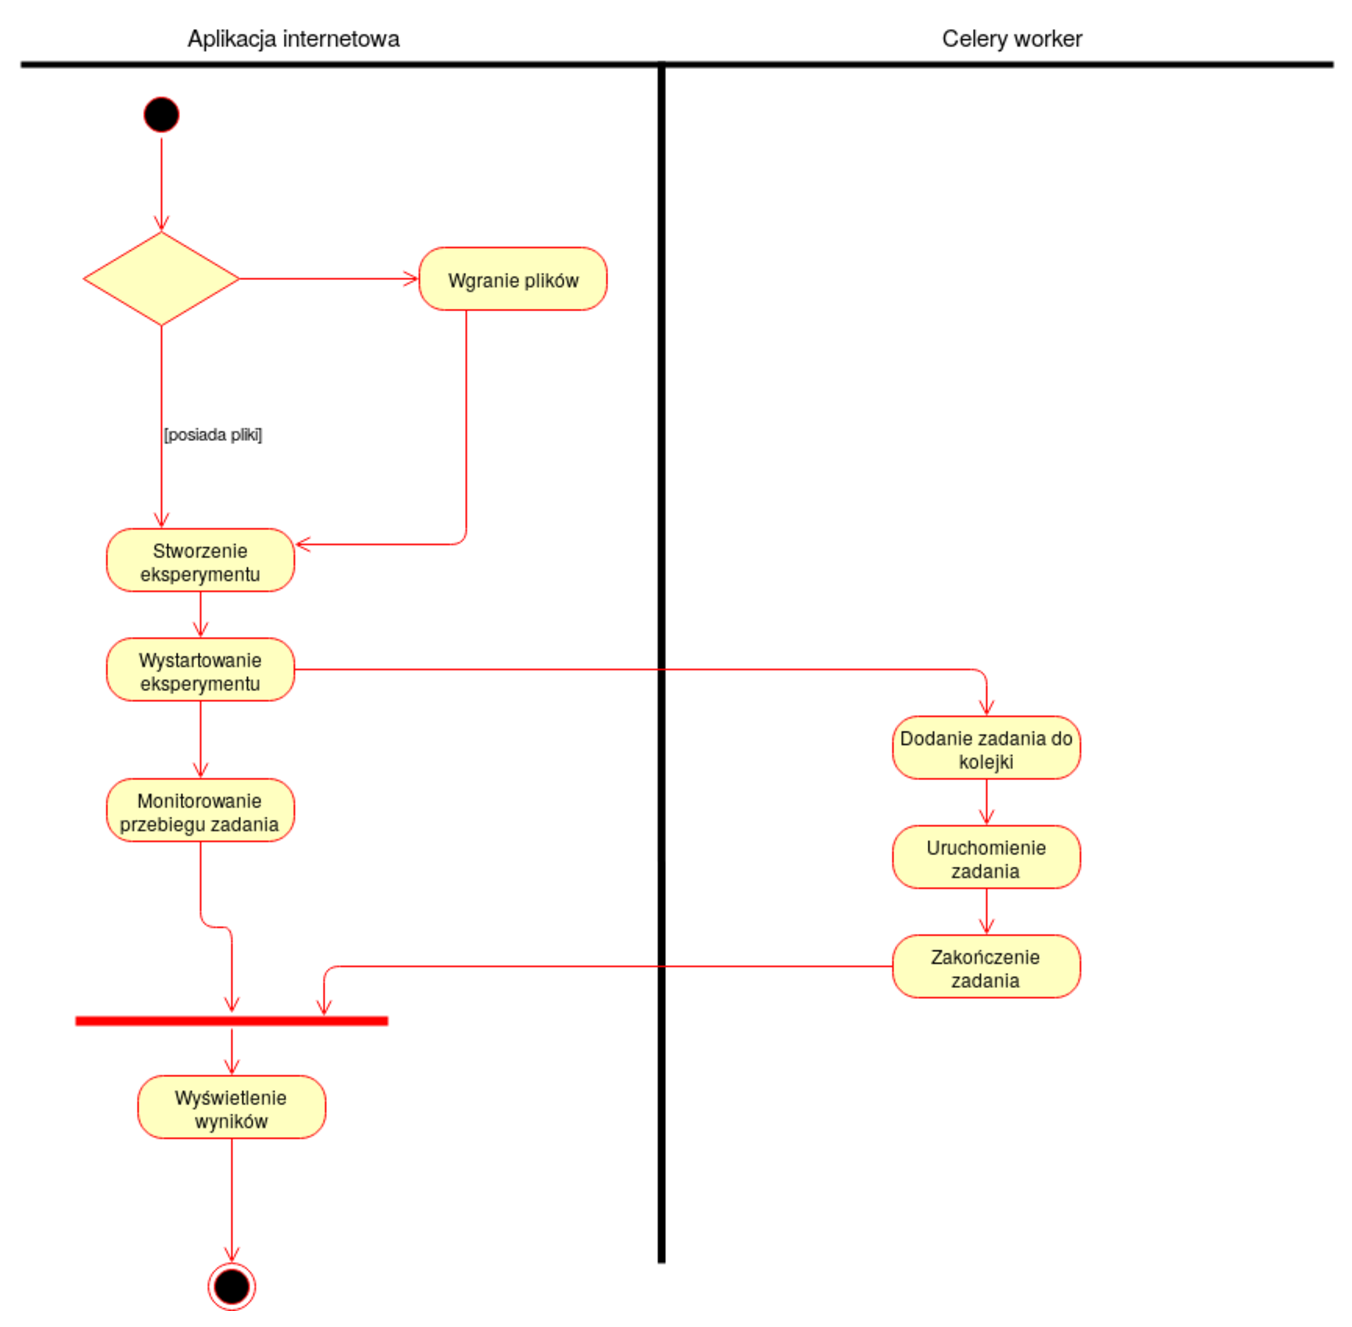
\includegraphics[width=11cm]{grafika/diagram_przebiegu_tworzenia_eksperymentu.eps}
	\caption{Diagram czynności tworzenia i uruchomiania eksperymentu, źródło: opracowanie własne}
	\label{rys2_diagram_czynności}
\end{figure}

Na rysunku \ref{rys1_diagram_przypadkow} przedstawiono wszystkie funkcjonalności w postaci diagramu przypadków użycia. W aplikacji zostały wyszczególnione trzy role dostępne do uzyskania dla każdego użytkownika oraz rola administratora całego systemu. Wszystkie przypadki użycia oprócz logowania i rejestracji są dostępne tylko dla użytkowników zalogowanych. Każdy nowy użytkownik musi założyć konto, aby mieć dostęp do aplikacji. Nowo powstałe konta otrzymują uprawnienia na domyślnym poziomie "1\_default", a wyższe poziomy uprawnień mogą zostać nadane po przez administratora. Kolejne role rozszerzają możliwości użytkownika pod względem ilości akcji możliwych do wykonania. Poziom "2\_exp"\ umożliwia tworzenie nowych eksperymentów, przy czym tylko najwyższy poziom uprawnień "3\_exp\_data"\  pozwala na wgrywanie plików do aplikacji. Przebieg czynności związanych ze stworzeniem nowego eksperymentu oraz wyświetleniem wyników został przedstawiony na rysunku \ref{rys2_diagram_czynności}. 



Opis przypadku użycia "Tworzenie nowego eksperymentu":
\begin{enumerate}
\item  Aktor
	\begin{itemize}
		\item Użytkownik. 
	\end{itemize}
\item Warunki początkowe
	\begin{itemize}
		\item Aktor jest zalogowany oraz posiada uprawnienia przynajmniej na poziomie "2\_exp".
	\end{itemize}
\item Zdarzenie inicjujące
	\begin{itemize}
		\item Naciśnięcie przycisku "New experiment" nad listą wszystkich eksperymentów użytkownika.
	\end{itemize}
\item Przebieg w krokach
	\begin{itemize}
		\item Aplikacja przechodzi do formularza tworzenia nowego eksperymentu,
		\item Użytkownik wypełnia i zatwierdza formularz.
	\end{itemize}
\item Przebiegi alternatywne
	\begin{itemize}
		\item  Użytkownik nie uzupełnia wszystkich pól formularza, aplikacja wyświetla powiadomienie o pustych polach.
	\end{itemize}
\item Sytuacje wyjątkowe
	\begin{itemize}
		\item  Użytkownik nie posiada żadnych plików wgranych do aplikacji. Powoduje to, że pola formularza zawierające pliki są puste. Uniemożliwia to stworzenie nowego eksperymentu, a aplikacja wyświetla powiadomienie o pustych polach przy podjętej próbie zatwierdzenia.
	\end{itemize}
\item Warunki końcowe
	\begin{itemize}
		\item  System przekierowuje użytkownika do listy z eksperymentami, a na liście znajduje się nowo utworzony eksperyment.
	\end{itemize}
\item Zależności czasowe
	\begin{itemize}
		\item  Częstotliwość wykonywania: Około 20 razy dziennie na każdego użytkownika,
		\item Typowy czas realizacji: 8 sekund.
	\end{itemize}
\end{enumerate}

Opis przypadku użycia "Wystartowanie eksperymentu":
\begin{enumerate}
	\item  Aktor
	\begin{itemize}
		\item Użytkownik. 
	\end{itemize}
	\item Warunki początkowe
	\begin{itemize}
		\item Aktor jest zalogowany oraz posiada stworzony eksperyment.
	\end{itemize}
	\item Zdarzenie inicjujące
	\begin{itemize}
		\item Naciśnięcie przycisku "Show" w liście eksperymentów na elemencie, którego status to "Created".
	\end{itemize}
	\item Przebieg w krokach
	\begin{itemize}
		\item Aplikacja przechodzi do podglądu szczegółów wybranego eksperymentu,
		\item Użytkownik klika przycisk "Start" znajdujący się na pasku możliwych czynności,
		\item Aplikacja przekierowuje użytkownika do listy eksperymentów.
	\end{itemize}
	\item Przebiegi alternatywne
	\begin{itemize}
		\item  Po wystartowaniu eksperymentu nastąpił błąd i jest to sygnalizowane zmianą statusu na "Error", a w szczegółach eksperymentu można podejrzeć wiadomość z błędem.
	\end{itemize}
	\item Sytuacje wyjątkowe
	\begin{itemize}
		\item  Użytkownikowi nie posiada prawd do wystartowania konkretnego eksperymentu i w panelu akcji nie wyświetla się przycisk Start".
	\end{itemize}
	\item Warunki końcowe
	\begin{itemize}
		\item  Eksperyment zmienił swój status na "In queue"\ lub "Running", a po przejściu do szczegółów wyświetla się pasek postępu oraz szacowany czas oczekiwania na zakończenie.
	\end{itemize}
	\item Zależności czasowe
	\begin{itemize}
		\item Częstotliwość wykonywania: Około 20 razy dziennie na każdego użytkownika,
		\item Typowy czas realizacji: 8 sekund.
	\end{itemize}
\end{enumerate}

Opis przypadku użycia "Wyświetlenie drzewa wynikowego":
\begin{enumerate}
	\item  Aktor
	\begin{itemize}
		\item Użytkownik. 
	\end{itemize}
	\item Warunki początkowe
	\begin{itemize}
		\item Aktor jest zalogowany oraz posiada ukończony eksperyment.
	\end{itemize}
	\item Zdarzenie inicjujące
	\begin{itemize}
		\item Naciśnięcie przycisku "Show" w liście eksperymentów na elemencie, którego status to "Finished".
	\end{itemize}
	\item Przebieg w krokach
	\begin{itemize}
		\item Aplikacja przechodzi do podglądu szczegółów wybranego eksperymentu, a na samym dole karty wyświetlają się linki do drzew decyzyjnych,
		\item Użytkownik klika w link do drzewa decyzyjnego.
	\end{itemize}
	\item Przebiegi alternatywne
	\begin{itemize}
		\item  Brak.
	\end{itemize}
	\item Sytuacje wyjątkowe
	\begin{itemize}
		\item  Brak.
	\end{itemize}
	\item Warunki końcowe
	\begin{itemize}
	\item  Aplikacja wyświetliła drzewo decyzyjne wraz ze statystykami.
	\end{itemize}
	\item Zależności czasowe
	\begin{itemize}
		\item Częstotliwość wykonywania: Około 30 razy dziennie na każdego użytkownika,
		\item Typowy czas realizacji: 10 sekund.
	\end{itemize}
\end{enumerate}

\section{Wymagania niefunkcjonalne}
asdasd.
\section{Wykorzystane technologie}
asdasd.
%\chapter{Przedstawienie problemu}

\section{Drzewa decyzyjne}

Podejmowanie decyzji jest procesem myślowym, który od początku istnienia ludzkości stwarza pewne trudności, a polega on na wybraniu najlepszego rozwiązania z dostępnych. Wpływ na optymalną decyzję mają informacje, które zostaną poddane analizie, ale także sama metoda analizy. Racjonalny wybór może być wspomagany różnymi algorytmami, czy też wizualną reprezentacją możliwych decyzji w postaci diagramu. Sam diagram może przybrać formę graficzną drzewa decyzyjnego.

Podstawowymi elementami drzewa są korzeń, gałęzie, węzły oraz liście. Korzeniem jest decyzja od którego rozpoczyna się budowa całej struktury zawierającej poszczególne węzły odpowiadające za sprawdzenie pewnego warunku. Natomiast gałęzie pełnią rolę połączenia wszystkich elementów \cite{misc_1}.  Liście są krańcowymi wierzchołkami drzewa i określają wybraną decyzje. Podczas próby określenia decyzji, należy poddać klasyfikacji posiadane dane, aby to osiągnąć konieczne jest przejście całego drzewa od samego korzenia do wynikowego liścia. Rezultatem takiej operacji będzie klasa definiująca decyzję.

\section{Uczenie maszynowe}
W otaczającym nas świecie ilość informacji produkowanych przez otoczenie oraz zbieranych przez firmy czy instytucje nadal przewyższa ilość danych, które można przeanalizować z użyciem obecnych zasobów. W celu wyciągnięcia wniosków z takiej ilości danych wykorzystuje się liczne rozwiązania technologiczne. Dzięki zastosowaniu różnych algorytmów przetwarzania danych, klasyfikacji oraz predykcji programy komputerowe posiadają możliwość uczenia się. Kierunek nauki, który zajmuje się tą dziedziną nazywamy uczeniem maszynowym. W ciągu ostatnich dziesięciu lat entuzjazm związany z wykorzystywaniem tej technologi wzrósł gwałtownie i w dużej mierze 
zdominował przemysł, ale również przyczynił się do jej rozwoju \cite{book_1}. Uczenie maszynowe stanowi trzon wielu usług, serwisów i aplikacji. Pod względem technologicznym odpowiada za wyniki wyszukiwania w przeglądarkach, za rozpoznawanie mowy przez nasze telefony, ale także jest odpowiedzialne za prowadzenie autonomicznych samochodów.

\section{Drzewa decyzyjne w technikach uczenia maszynowego}

Drzewa decyzyjne stanowią jedne z bardziej wszechstronnych algorytmów w  dziedzinie uczenia maszynowego. Z jednej strony mogą być wykorzystywane w zadaniach z zakresu klasyfikacji, a z drugiej strony również odgrywają ważną rolę w regresji \cite{book_1}. Z ich pomocą możemy uzyskać potężne modele i narzędzia zdolne do uczenia się ze złożonych zbiorów danych. Dodatkowym atutem drzew jest możliwość wizualnego przedstawienia rozwiązania, które będzie zrozumiałe dla osób nie mających do czynienia z uczeniem maszynowym lub ze statystyką. Z racji wzrostu popularności tej technologi zwiększyły się nakłady pracy naukowej w celu osiągnięcia coraz to lepszych i bardziej optymalnych algorytmów pod względem wydajnościowym. 

\subsection{System GDT}
Pracownicy Politechniki Białostockiej również mają wkład w budowę takich rozwiązań. Autorski system GDT (\textit{Global Decision Trees}), który jest wykorzystywany w aplikacji inżynierskiej, służy do generowania modelu drzewa decyzyjnego na podstawie zbiorów wejściowych. Ten system jest zaimplementowany w języku c++ oraz jest skompilowany do pliku wykonywalnego, aby umożliwić jego uruchomianie z poziomu konsoli systemu operacyjnego. Całe rozwiązanie jest unikalne, a głównym założeniem jest wykorzystanie algorytmów genetycznych. Z ich pomocą przestrzeń rozwiązań danego problemu jest większa niż w klasycznym podejściu, co skutkuje możliwością osiągnięcia dokładniejszych i lepszych wyników. Metody pracy algorytmów genetycznych w dużej mierze odwzorowują działania samej natury \cite{book_2}. Podczas definiowania pracy algorytmu należy podać takie parametry jak wielkość populacji, prawdopodobieństwo mutacji czy też krzyżowania się danych osobników. Wartości tych parametrów i innych są określane w pliku konfiguracyjnym opartym o strukturę XML, który jest zarazem plikiem wejściowym do aplikacji GDT. System oprócz tego pliku wykorzystuje pliki z konkretnymi rozszerzeniami:
\begin{itemize}
	\item *.data - plik zawierający dane treningowe, 
	\item *.test - plik zawierający dane testowe,
	\item *.names - plik określających nazwy klas oraz rodzaj zmiennych.
\end{itemize}
Na podstawie tych danych aplikacja GDT może stworzyć model drzewa decyzyjnego, którego przedstawienie jest zapisywane w pliku tekstowym. 

\section{Istniejące rozwiązania}
Aktualnie na rynku znajduje się mała liczba rozwiązań oferujących tworzenie drzew decyzyjnych. Aplikacje, które można wyróżnić różnią się między sobą zakresem funkcjonalności. Rozwiązania internetowe głównie są oparte o zarobek pieniężny, ale oferują też darmowe wersje z pewnymi ograniczeniami. Istnieją też liczne rozwiązania dla programistów w postaci paczek możliwych dla każdego z popularniejszych języków. Biblioteki te umożliwiają w prosty sposób stworzenie podstawowych modeli uczenia maszynowego w tym drzew decyzyjnych. Negatywną cechą takiego rozwiązania jest wymagana przynajmniej podstawowa wiedza z zakresu programowania u użytkownika. Dodatkowo chcąc osiągnąć bardzo wydajne modele trzeba dokładnie znać mechanizmy działające pod strukturą biblioteki. Występują również nie liczne rozwiązania desktopowe. W głównej mierze są one rozwijane przez uniwersytety. Do wykonania obliczeń wymagają dość przyzwoitego sprzętu komputerowego, który umożliwi optymalną moc obliczeniową.    

\begin{figure}[htb]
	\centering
	\includegraphics[width=11cm]{grafika/smartdraw.eps}
	\caption{Strona główna aplikacji \textit{SmartDraw}.}
	\label{rys21_smartdraw}
\end{figure}

\begin{figure}[htb]
	\centering
	\includegraphics[width=11cm]{grafika/smartdraw_tree.eps}
	\caption{Drzewo stworzone w aplikacji \textit{SmartDraw}.}
	\label{rys22_smartdraw_tree}
\end{figure}


Aplikacja internetowa \textit{SmartDraw} jest jedną z wygodniejszych platform do tworzenia diagramów \cite{misc_smartdraw}. Dostęp do platformy następuje po przez przeglądarkę internetową. Założenie konta jest darmowe wraz z okresem próbnym. Po pewnym czasie aplikacja wymaga opłacenia miesięcznego abonamentu. Widok strony głównej został przedstawiony na Rys. \ref{rys21_smartdraw}. Platforma ponadto udostępnia funkcjonalność tworzenia innych rodzajów diagramów. Proces budowy nowego schematu przebiega po przez przeciągnie i łączenie bloków. Istnieje również wczytanie struktury drzewa z pliku o rozszerzeniu *csv. Grafy są prezentowane w czytelny i przyjemny dla oka sposób (Rys. \ref{rys22_smartdraw_tree}). Ukończony diagram można wyeksportować do pliku graficznego lub dokumentu programu Word. Aplikacja niestety nie umożliwia analizy informacji przy pomocy jakiegoś algorytmu. Skutkuje to brakiem opcji zbudowania drzewa decyzyjnego w pełni opartego o pliki ze zbiorami danych. 

\begin{figure}[htb]
	\centering
	\includegraphics[width=11cm]{grafika/canva.eps}
	\caption{Strona główna aplikacji \textit{Canva}.}
	\label{rys23_canva}
\end{figure}

\begin{figure}[htb]
	\centering
	\includegraphics[width=11cm]{grafika/canvas_tree.eps}
	\caption{Drzewo stworzone w aplikacji \textit{Canva}.}
	\label{rys24_canva_tree}
\end{figure}

\textit{Canva} to kolejne narzędzie umożliwiające na tworzenie drzew decyzyjnych przy pomocy przeglądarki internetowej \cite{misc_canva}. Dostęp do platformy wymaga założenia konta i daje możliwość tworzenia projektów graficznych. Aplikacja posiada również rozszerzenia funkcjonalności przy pomocy pakietów płatnych dla firm jak i osób prywatnych. Strona główna aplikacji została przedstawiona na Rys. \ref{rys23_canva}. Użytkownik ma możliwość tworzenia drzewa tylko po przez przeciąganie konkretnych elementów. W aplikacji brakuje opcji wyliczenia drzewa na podstawie zbioru danych i wybranego algorytmu. Tworzone diagramy można wzbogacić o liczne walory wizualne i dostępne gotowe motywy (Rys. \ref{rys24_canva_tree}). Głównymi odbiorcami aplikacji są reklamodawcy oraz osoby prowadzące rozbudowaną działalność w serwisach społecznościowych.  
 
\begin{figure}[htb]
	\centering
	\includegraphics[height=7cm]{grafika/weka.eps}
	\caption{Okno główne aplikacji \textit{Weka}.}
	\label{rys25_weka}
\end{figure}

\begin{figure}[htb]
	\centering
	\includegraphics[width=11cm]{grafika/weka_tree.eps}
	\caption{Drzewo stworzone w aplikacji \textit{Weka}.}
	\label{rys26_weka_tree}
\end{figure}

\textit{Weka} jest narzędziem desktopowym stworzonym przez pracowników zajmujących się tematami uczenia maszynowego na Uniwersytecie Waikato w Nowej Zelandii. Aplikacja została zaimplementowana przy pomocy języka programowania Java. Dzięki temu platforma natywnie może działać na każdym systemie operacyjnym. Główne okno aplikacji zostało zaprezentowane na Rys. \ref{rys25_weka}. Posiada także liczne wrappery umożliwiające korzystanie z zaimplementowanych mechanizmów za pośrednictwem różnych języków programowania. Przy pomocy aplikacji użytkownika ma dostęp do dużej ilości algorytmów klasyfikacji z wykorzystaniem uczenia maszynowego, łącznie z drzewami decyzyjnymi. Tworzenie nowego eksperymentu zaczyna się od wybrania zestawu danych. Użytkownik początkujący może skorzystać z przykładowych plików. Po wczytaniu zbioru istnieje możliwość podejrzenia wizualizacji danych oraz ich wstępna obróbka. W kolejnym kroku użytkownika musi wybrać interesujący sposób klasyfikacji, do wyboru jest kilka różnych algorytmów związanych z tworzeniem drzew decyzyjnych, ale i nie tylko. Proces obliczeń może zająć chwile czasu i zależy głownie od ilości danych oraz zasobów mocy obliczeniowej. Rezultaty eksperymentu są przedstawione w postaci przedstawionej, ale także istnieje opcja wyświetlenia grafu. Przykładowe drzewo decyzyjne stworzone za pośrednictwem programu zostało przedstawione na Rys. \ref{rys26_weka_tree}. Ponadto poszczególne atrybuty węzłów zostają zobrazowane za pośrednictwem wykresów. Aplikacja umożliwia również liczne modyfikacje w parametrach algorytmów.  



Rozwiązanie oferowane przez pracę dyplomową jest unikalne nie tylko ze względu na wykorzystany system GDT. Wyróżnia się w pełni niezależnością użytkownika od sprzętu, który posiada, co w przypadku takich rozwiązań jak program \textit{Weka} ma znaczenie. Aktualnie dostępne rozwiązania internetowe nie wyróżniają się miedzy sobą,a dodatkowo umożliwiają ograniczone funkcjonalności co do budowania drzew na podstawie zbiorów danych. 
\nocite{*} %wszystkie wpisy w bibliografi
\bibliographystyle{unsrt} %{latex8} posortowane wzgledem wystepowania
\bibliography{bibliografia}%

\addtocontents{toc}{\contentsline {chapter}{Bibliografia}{\thepage}{}}
\listoftables
\addtocontents{toc}{\contentsline {chapter}{Spis tabel}{\thepage}{}}
\listoffigures
\addtocontents{toc}{\contentsline {chapter}{Spis rysunk�w}{\thepage}{}}
\lstlistoflistings
\addtocontents{toc}{\contentsline {chapter}{Spis listing�w}{\thepage}{}}
\listofalgorithms % w zaleznosci od kompilatora i wersji klasy moga wystapic bledy przy kompilacji
\addtocontents{toc}{\contentsline {chapter}{Spis algorytm�w}{\thepage}{}}

%\biblioteka{tak} % tak/nie
\end{document}
